\documentclass[12pt]{article}
\usepackage{lscape}
\usepackage{amsmath}
\usepackage[sort]{natbib}
\usepackage{setspace}
\usepackage{graphicx}
\usepackage{lscape}
\usepackage{isorot}
\usepackage{booktabs}
\usepackage[print,sectionbreak,panelright]{pdfscreen}
\usepackage{hyperref}
\usepackage{array}
\usepackage[cmbold]{mathtime}
\usepackage{amsmath}
\usepackage[sort]{natbib}
\usepackage{xspace}
\usepackage{graphicx}
\usepackage{hyperref}

\newcolumntype{H}{>{\setbox0=\hbox\bgroup}c<{\egroup}@{}}
\doublespacing
\newcolumntype{H}{>{\setbox0=\hbox\bgroup}c<{\egroup}@{}}
\usepackage{lscape}
\setlength{\textwidth}{6.5in}
\setlength{\textheight}{9.0in}
\setlength{\oddsidemargin}{0in}
\setlength{\topmargin}{0.0in}
\setlength{\headheight}{0in}
\setlength{\headsep}{0.0in}
\usepackage{lscape}
\usepackage{amssymb}
\usepackage[margin=0.7in]{geometry}
\newcolumntype{H}{>{\setbox0=\hbox\bgroup}c<{\egroup}@{}}
% code that creates meaningful variable names from the short stata names
\usepackage{graphicx,amsmath}
\usepackage{epsfig}

\topmargin=-.5in \oddsidemargin=0in \textwidth=6.5in
\textheight=9in

\parindent 0.0in
\parskip .20in

\def\balpha{\pmb{\alpha}}
\def\bbeta{\pmb{\beta}}
\def\bgamma{\pmb{\gamma}}
\def\bdelta{\pmb{\delta}}
\def\bmu{\pmb{\mu}}
\def\bsigma{\pmb{\sigma}}
\def\bphi{\pmb{\phi}}
\def\bTheta{\pmb{\Theta}}
\def\btheta{\pmb{\theta}}
\def\btau{\pmb{\tau}}
\def\bomega{\pmb{\omega}}

\def\bX{\pmb{X}}
\def\bY{\pmb{Y}}
\def\bZ{\pmb{Z}}
\def\bJ{\pmb{J}}
\def\bV{\pmb{V}}
\def\bR{\pmb{R}}
\def\bW{\pmb{W}}





\begin{document}

\title{Hierarchical Bayes models for daily rainfall time series at multiple locations from different data sources\\
%\thanks{ thanks...}
}
\author {Kenneth Shirley \thanks{ATT Research Labs}
\and Kathryn Nadine Vasilaky \thanks{Earth Institute and International Research Institute for Climate and Society, Columbia University, Lamont Campus 61 Route 9W, Lamont Hall, 2G (corresponding email: \tt{knv4columbia.edu})}
\and Daniel Osgood \thanks{International Research Institute for Climate and Society Columbia University}
\and Helen Greatrix  \thanks{International Research Institute for Climate and Society Columbia University}

}
\maketitle

\vspace{-4ex}

\begin{singlespace}  
\begin{abstract}

We estimate a Hierarchical Bayesian models for daily rainfall that incorporates two novelties for estimating spatial and temporal correlations. We estimate the within site time series correlations for a particular rainfall site using multiple data sources at a given location, and we estimate the across site covariance in rainfall based on location distance. Previous models have captured cross site correlations as a functions of site specific distances, but not within site correlations across multiple data sources, and not both aspects simultaneously. Further, we incorporate information on the technology used (satellite versus rain gauge) in our estimations, which is also a novel addition. This methodology has far reaching applications to other data contexts in which multiple datasources exist for a given event or variable for which within and between site covariances can be estimated over time. 

\end{abstract}


\thispagestyle{empty}
%\vspace{1em}
\noindent JEL Classification: O160, G22, Q140\\
\noindent Keywords: micro finance, index insurance, credit constraints, financial education 
\end{singlespace}
 
\newpage

%subsidized=liquidity relaxation



\section{Motivation}

Weather simulations are used to study future weather patterns in the context of climate-sensitive systems, and to simulate climate change scenarios and study its repercussions. Extreme weather events, such as drought, are frequently the hardest to predict,  the most damaging to agricultural livelihoods and the costliest events in terms of disaster response. However, multiple data sources may not always coincide with one another and may not coincide with human experience of extreme weather events making responsiveness difficult. In the case of such conflicting data, it is important that weather predictions are not drawn based on one information source alone, but with attention to multiple sources and the technology with which data are captured. Futhermore, more robust within site estimations can render more robust across site correlations. Both aspects can enable better simulation. 

Past weather simulators have not simultaneously captured within site and across site correlation of weather time series. Initially, many weather simulators were estimated using one time series per location. 
%history: markov, distributions, multiple sites, h bayes
Wilks and Wilby (1999) provide an overview of the developments in weather simulation. Weather series were first modeled with stochastic point process models in space and time. Both (Sanso) and (weather game) provide good overviews of this trajectory. First order Markov chains were first used to generate such point processes, modeling the occurrence of rainy versus non-rainy days dictated by transition probabilities. Transition probabilities were based on the relative frequency of precipitation in observed climatology (Gabriel and Neumann (1962)). Improvements to this first model then included modeling the non-zero rainfall days (Todorovic and Woolhiser, 1975), which followed with developments in the type of distribution for non-zero days: including an exponential distribution (Richardson (1981)) and then a gamma distribution [Thom, 1958; Katz, 1977; Buishand, 1977; 1978; Stern and Coe, 1984; Wilks, 1989; 1992 (1981)]. Other methodologies for simulating precipitation occurrences is the use of spell-length models. Rather than simulating rainfall occurrences day by day, spell-length models operate by fitting wet and dry periods to different probability distributions (Buishand, 1977; 1978; Roldan and Woolhiser,1982). Non-parametric simulation methods have also been developed which involved resampling data such that time correlations are captured in the resampling to estimate distribution parameters (Young (1994), Lall and Sharma (1996), Lall et al. (1996) and Rajagopalan et al. (1997)).
	
The objective in all of these approaches is to be able to simulate long synthetic time-series of weather that reflect key observed statistics in the region of interest e.g. means, dry spell lengths, inter annual rainfall variability, or probability of extreme events occurring. Capturing a spatial dependence between sites or series, as well as charactersitics of the series themselves, such as non-stationarity, can improve our predictive analytics. 

%spatial motivation
Thus incorporating observed spatial correlations into a well calibrated stochastic approach is likely to lead to more realistic impact models.  Several different techniques and methods have been suggested.  The MarkSim weather generator uses spatially correlated input grids of statistics to allow one to allow estimation at a site where there are no observations (Jones and Thornton, 1993). Wilks (1999,1998) extended a Richardson weather generator by driving it with a grid of spatially correlated random numbers.  More recently this approach was extended in the GIST weather generator, which incorporates spatial correlation through the use of correlation matrices to sample from a cumulative probability function at each location (Baigorria and Jones, 2010), or in Kleiber et al (2012) the use of latent Gaussian processes. In 2012. Greatrex (2012) proposed a geostatistical sequential simulation approach coupled to a markov generator, which would allow spatially correlated ensembles of maps of rainfall to be generated.  It is important to note that many of these approaches rely on a large amount of observed and calibrated data, for example a dense station network to create variograms [HELEN EXPLAIN].   

Hierchacal bayesian estimation is yet another approach equipped to model spatial as well as temporal relationships. It goes beyond the simplistic and often linear relationships assumed in markovian weather simulators. It models and estimates the functional relationship between weather series over time. The most recent development in the use of the hierarchal bayesian approach comes from Sanso and Guenni (2012), which improves upon Sanso and Duenni (1996), by 1) incorporating spatial correlation for the joint distribution of weather series from several stations and 2) the non-stationarity of rainfall data. The authors show that their model is able to simulate weather data and summary statistics for a large number of stations, some of which have poor quality data. 

While we do not focus on the aspect of non-stationarity aspect in raifnall series, the novelty of our approach is our ability to account for two levels of the rainfall time series information at each site: 1) both the location of the measurement and 2) the instrument used to measure rainfall are incorporated. In addition, we 3) estimate the the spatial covariance between all these series and 4) the noise or error in recording rainfall due to the instrument itself. By incorporating several layers of information sources for each site in which we would like to predict weather, we are adding more information to the parameter estimates and, hopefully, improving out-of-sample predictions. Because we used daily data to fit our model, our simulated data and out-of-sample predictions are daily, which allows us to compute statistics sensitive to daily measurements: probability of rainfall, dry spells, and extreme rainfall. 

The ability to incorporate spatial correlations has several policy implications. First, food insecurity is generally correlation in time and space in parallel with rainfall patterns. Thus, predictions that incorporate these patterns can allow for better response to anticipated droughts and subsequent food shortages. This is crucial for aid organizations and first responders to such crises. In addition, longer term tools such as weather insurance, are quite sensitive to spatial phenomena. Higher spatial correlations affect the price and responsiveness of such financial tools. Large covariate risks are the focus of index insurance, for example, and institutions offering such tools need adequate capital holdings to properly respond to the degree of and size of covariate risk. 


The remainder the paper is as follows. In In Section~\ref{sec:data} describes the data used and its preparation. In Section~\ref{sec:model} shows how rainfall the and the processes are modeled in a  hierarchical fashion. In Section~\ref{sec:fit} discusses the parameters to be estimated. In Section~\ref{sec:sim} exhibits the performance in recovering parameters with simulated data. In Section~\ref{sec:validate} exhibits the ability of our model,  using our real historical data, in recovering deliberately removed portions of the data. In Section~\ref{sec:results}  we graph the posteriors distributions for select parameters using the full historical data set. In Section~\ref{sec:discuss} concludes and describes next steps. 



%More recently, simulators aim to generate weather sequences at multiple points, where the spatial correlations between rainfall occurrence at different sites are captured using spatially dependent random variables (Wilks 1999). More recently Yatest et al (2003) and later Apipattanavis et. al. (2007) model  spatially averaged weather time series for a representative time series of an entire region. As the authors, state, this approach works well if the sites are homogenous in terms of their weather. 

%Crop yields respond to rainfall and temperature, but average decadal or even average monthly rainfall can obscure the effects of weather on yields. Frequent exposure to extreme temperatures (high and low) matters tremendously (Schlenker 2009). Furthermore, the daily variation in other variables, such as soil moisture, has been found to be equally important, and if not accounted for, allows for temperature's effect to be overstated (Ortiz 2014). Specifically, the NUMBER of times and WHEN a crop is exposed to highs/lows in temperature and moisture is crucial, which decadal or monthly measures cannot capture. [Is this disingenuous if we don't have temperature but just rainfall amount?]

%Daily statistics and extremes of weather often have a greater impact on end-users than climatological averages. For example, although seasonal rainfall totals and average temperatures can provide a general guide to crop yields, plants are also extremely sensitive to extreme weather events over a few hours (Schlenker, 2009, Ortiz 2014), especially during flowering or pod-set.  A classic example is in groundnut, where high temperatures during the one or two days of flowering leads to pod death and plant death (Wheeler et al, 1996; Wheeler et al, 2000), or in maize, where a dry spell over the short Anthesis Tasselling Interval has a well measured and catastrophic impact on yields (Bola�os and Edmeades (1996)).  Similar impacts can be seen in hydrology, where extreme rainfall events that are often of more interest to flood modelers than seasonal averages \citet{hydro}, or in climate science, where it is crucial to be able to convert projections of regional averages into changes in local weather (REFERENCE).    

%The ability to generate realistic daily time-series of weather is therefore valued in many end-user applications such as hydrological, climate or crop simulation modeling, especially over regions of the world where there are sparse ground based weather station networks.  




\section{Procedure and Data}
\label{sec:data}

We model a set of 15 time series of daily rainfall in Ethiopia during the time period from 1992 to 2010, where these 15 time series come from six different locations, and each location has at least two time series of daily rainfall associated with it. The reason we observed multiple time series for each location is that for each location we have multiple sources of data, including rain station data and satellite-based rainfall proxy data. The statistical challenge to modeling such data is to separately estimate the spatial variability between locations and the within-location measurement-based variability. A standard hierarchical model with sets of 15 exchangeable parameters -- one for each time series -- would conflate these two sources of variation. The model we introduce here -- a hierarchical Bayesian model with one level for locations, and another level for multiple data sources within a location -- explicitly models each of these two sources of variation.

Figure~\ref{fig_ethiopia_map} shows the six locations from which the daily rainfall time series are measured. The names of the locations are Hagere Selam, Maykental, Mekele, Abi Adi, Agibe, and Adi Ha. The last of these, Adi Ha, is the location we are most interested in, because we wish to provide rainfall insurance for farmers who live there. Specifically, we want to model rainfall at one of the automated rain stations at Adi Ha, which is one of the 15 time series in our data set, but is also the series that has the least amount of observed data -- only about 200 days worth of data from 2009.

\begin{figure}[htbp]
\begin{center}
\includegraphics[width=4.5in]{fig_ethiopia_papermap.jpg}
\caption{A map of the 6 locations, where the green squares denote ARC pixels and the pins denote rain station locations. The inset in the upper right corner shows the area of the map with a red rectangular box; this region is in north central Ethiopia.}
\label{fig_ethiopia_map}
\end{center}
\end{figure}

The specifics of the data are as follows:
\begin{itemize}
\item For the first five locations, we have rain station data as well daily measurements from a satellite product called ARC, which is a rainfall proxy based on the temperature of the clouds over an area of about one hundred square kilometers. This comprises $ 5 \times 2 = 10$ time series.
\item For the sixth location, Adi Ha, we have five separate data sources:
\begin{enumerate}
\item One reliable rain station from which we only have 200 days of data from 2009-2010; this is the time series in which we have the most interest, because it is a new, accurate rain station on which we want to base insurance contracts.
\item One unreliable rain station from which we have about 7 years of data from 2000-2009, with about 2 years of missing data interspersed.
\item The ARC satellite proxy.
\item Two additional satellite proxies that are different from ARC.
\end{enumerate}
\end{itemize}

Figure~\ref{fig_overlap} shows the range of observed and missing data for each of these 15 time series; note that the time scale goes back to 1961 for one of the rain stations, but for simplicity, we only consider the time span of 1992-2010 in our model fit, because this span contains most of the data.

\begin{figure}[htbp]
\begin{center}
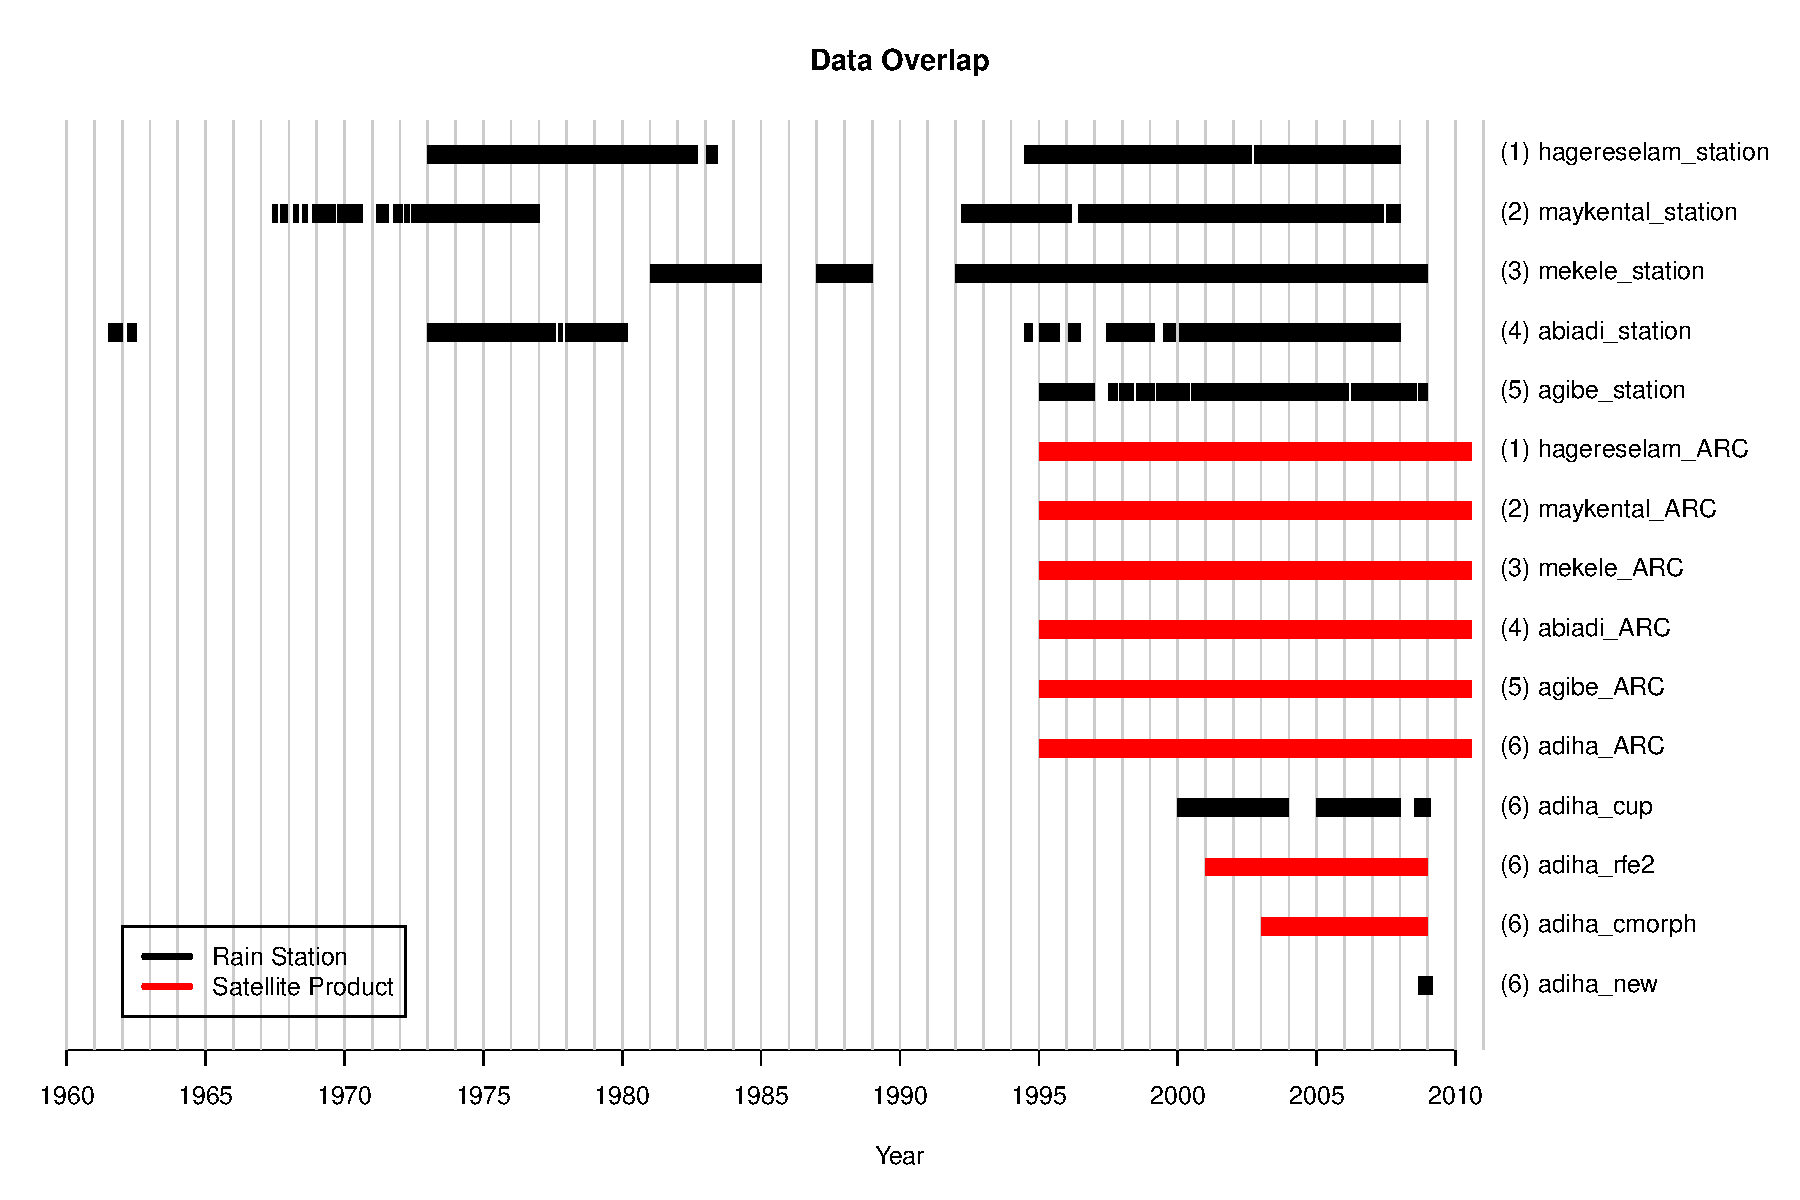
\includegraphics[width=5.0in]{fig_observed_data_new.pdf}
\caption{A visualization of the observed data for each of the 15 time series we model. The black hash marks denote rain station data, and the red hash marks denote satellite-based data.}
\label{fig_overlap}
\end{center}
\end{figure}

Table~\ref{tab_summary} contains some background information and summary statistics related to each time series of daily rainfall. For each time series we record the latitude, longitude, and elevation of the location where measurements were made, and the number of days of observed data. The maximum distance between locations is about 70 kilometers (between Mekele in the southeast and Maykental in the northwest).
\begin{table}[htdp]
\caption{Background information about the 15 time series}
\begin{center}
\begin{tabular}{|l|l|l|l|r|r|}
\hline
 & Site & Latitude & Longitude & Elev. (m) & Num. Obs \\
\hline
1 & Hagere Salaam & $13^\circ$ 38' 49'' & $39^\circ$ 10' 19'' & 2625 & 4887 \\
2 & Hagere Salaam (ARC) & '' & '' & '' & 5632 \\
3 & Maykental & $13^\circ$ 56' 13'' & $38^\circ$ 59' 49'' & 1819 & 5620 \\
4 & Maykental (ARC) & '' & '' & '' & 5632 \\
5 & Mekele & $13^\circ$ 28' 1'' & $39^\circ$ 31' 1'' & 2247 & 6205 \\
6 & Mekele (ARC) & '' & '' & '' & 5632 \\
7 & Abi Adi & $13^\circ$ 37' 19'' & $39^\circ$ 0' 10'' & 1849 & 4205 \\
8 & Abi Adi (ARC) & '' & '' & '' & 5632 \\
9 & Agibe & $13^\circ$ 33' 43'' & $39^\circ$ 3' 43'' & 1952 & 4722 \\
10 & Agibe (ARC) & '' & '' & '' & 5632 \\
11 & Adi Ha (ARC) & $13^\circ$ 43' 48'' & $39^\circ$ 05' 38'' & 1713 & 5632 \\
12 & Adi Ha (Rain Station - Manual) & '' & '' & '' & 2769 \\
13 & Adi Ha (RFE2) & '' & '' & '' & 2920 \\
14 & Adi Ha (CMorph) & '' & '' & '' & 2190 \\
15 & Adi Ha (Rain Station - Automatic) & '' & '' & '' & 186 \\
\hline
\end{tabular}
\end{center}
\label{tab_summary}
\end{table}%

\subsection{Exploratory Data Analysis}

In this part of Ethiopia, the rainy season lasts roughly from June to October. Figure~\ref{fig_eda} shows the percentage of rainy days and the average amount of rain as a function of the time of year for each time series. The basic modeling strategy will be to use a set of periodic functions to model rainfall as a function of the season of the year.
\begin{figure}[ht]
\begin{center}
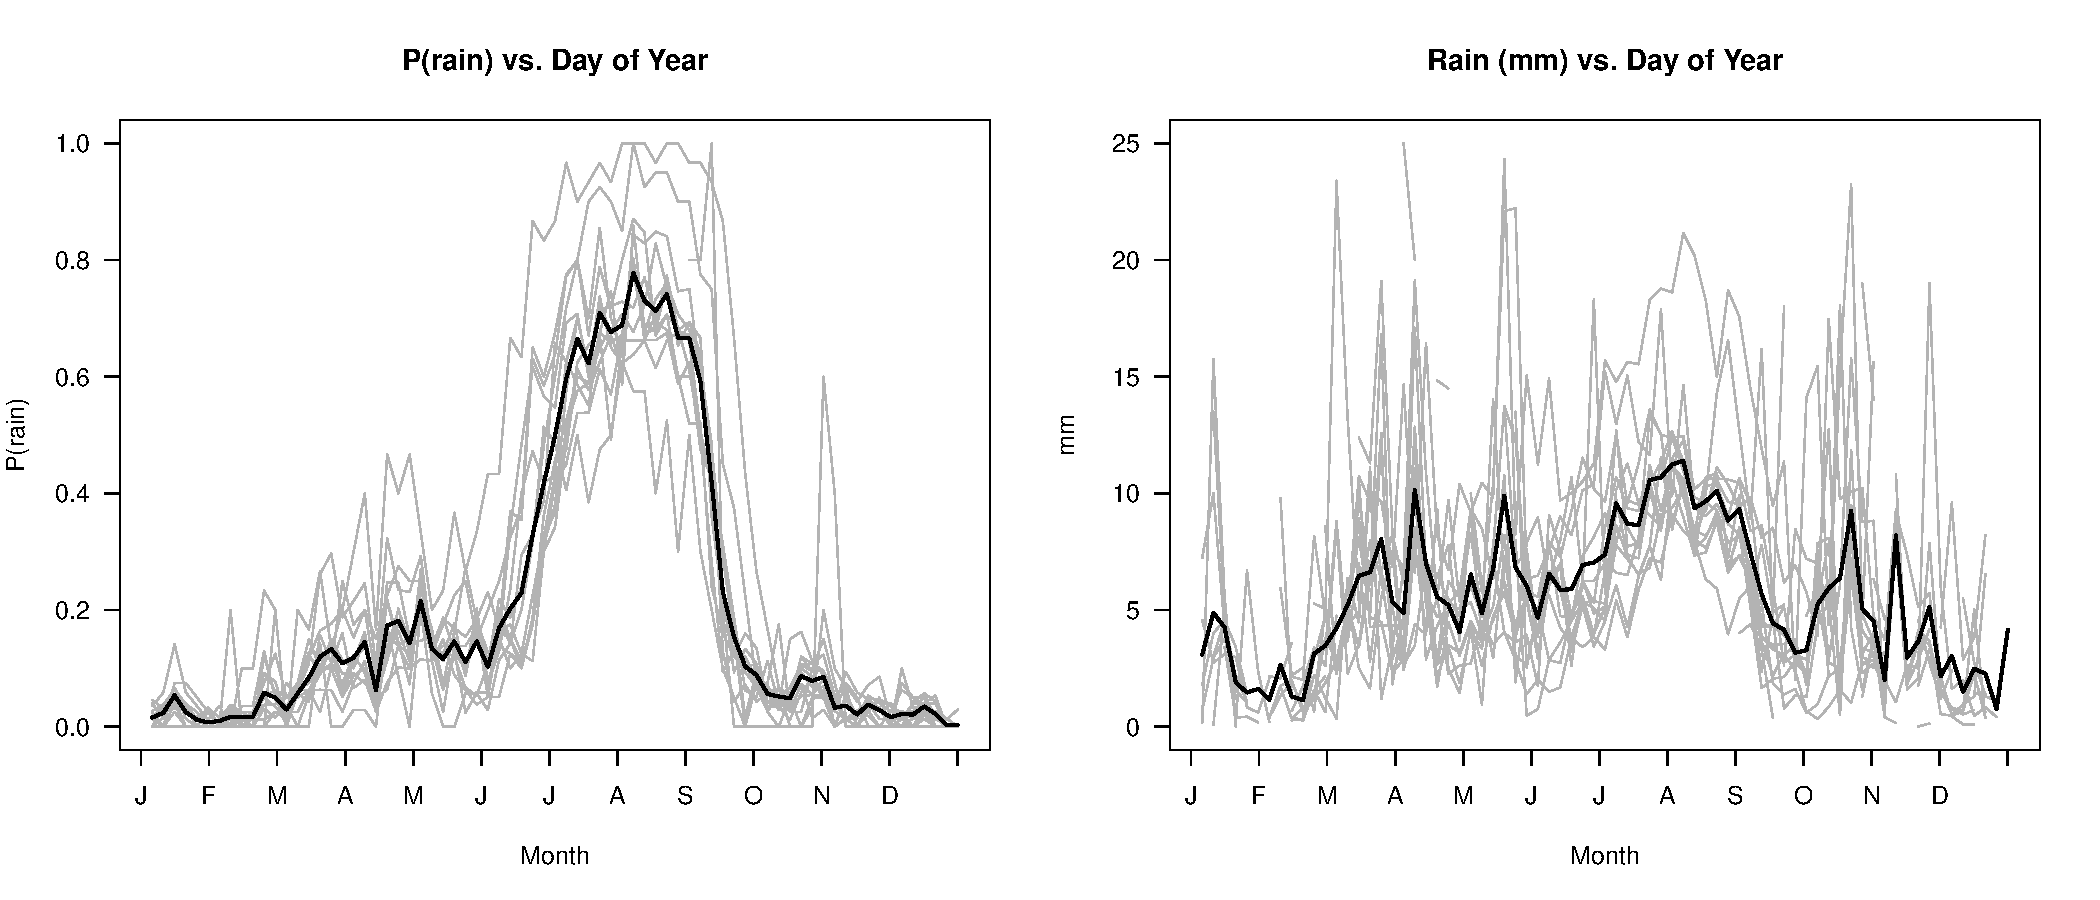
\includegraphics[width=6.5in]{fig_eda.pdf}
\caption{Plots of the percentage of rainy days (pooled into 5-day bins) and the average amount of rain as a function of the season. The gray lines are for each of the 15 individual time series, and the black lines are averaged across all 15 time series.}
\label{fig_eda}
\end{center}
\end{figure}

We are also interested in the difference, on average, between the measurements of rainfall based on the ARC satellite proxy and the rain stations. Comparing rainfall frequencies pooled over 5-day periods, averaging across all parts of the year and all five locations with exactly one rain station and one ARC measurement, we find that the ARC records about 3\% fewer days of rainfall than the rain stations. Across locations, this difference ranges from about -6\% (Hager Selam) to  +1\% (Agibe).



\section{Modeling Rainfall}
\label{sec:model}
%Our model consists of two main components: a model for the binary variable of whether or not it rains on a given day (called the frequency model), and a model for the amount of rainfall, given that there was rainfall (called the intensity model). In this paper, we are most interested in the frequency model; the methods we use to model frequency, though, could also be used to model intensity.

We fit a tobit model for daily rainfall at multiple locations, with multiple time series observed at each site. Let us first set up some notation. Let $S=6$ denote the number of locations where we measure rainfall, and $\bJ = \{2,2,2,2,2,5\}$ is the vector denoting the number of daily rainfall time series observed for each of the $S$ locations. The total number of days in our time series is $N=6679$ days, from 1/1/1992 through 7/28/2010. Let $Y_{stj}$ denote the amount of rainfall, measured in mm, for location $s \in (1,...,S)$, day $t \in (1,...,N)$, and time series $j = (1,...,J_s)$. Last, let $D_{ik}$ denote the Euclidian distance between site $i$ and $k$, for $i,k \in (1,...,S)$.

We model $Y_{stj}$ using a hierarchical Bayesian tobit regression model, where the levels of the hierarchy correspond to different sources of variation:

% observations:
$\hspace{0.5in}
Y_{stj} = \begin{cases} W_{stj} &\mbox{if } W_{stj} > 0 \hspace{2.5in} \text{Observed rainfall}\\
0  &\mbox{if } W_{stj} \leq 0, \end{cases}
$

% Latent continuous rainfall
$\hspace{0.9in}
\bW_{st} \sim \text{N}_{J_s}(\bZ_{st} + \bX^\text{ARC}_s \beta^\text{ARC}_s, \frac{1}{\gamma_{st}}\Sigma_s), \hspace{1.55in} \text{Latent rainfall}
$

% Underlying spatial mean rainfall process for each location:
$\hspace{1.3in}
\bZ_t \sim N_S(\bX_t \bbeta^Z, \tau^2\bV), \hspace{1.75in} \text{Spatial mean rainfall}
$

% covariates including linear, quadratic time, sine and cosine, plus nino by month:
$\hspace{1.7in}
\beta_{ps}^Z \sim \text{N}(\mu_p, \sigma^2_p),
$

% mean of the groups of coefficients across locations
$\hspace{2.1in}
\mu_{p} \sim \text{N}(0, 5^2),
$

% variance of the groups of coefficients across locations
$\hspace{2.1in}
\sigma_{p} \sim \frac{1}{2}\text{t}(0, 1, \text{df} = 3),
$

% 'nugget effect' of spatial covariance:
$\hspace{1.7in}
\tau \sim \frac{1}{2}\text{t}(0, 1, \text{df} = 3),
$

% parametric spatial covariance matrix, exponential model
$\hspace{1.7in}
\bV=\{v_{ik}\}, v_{ii}=1, v_{ik} = \exp(-\lambda d_{ik}) \hspace{0.3in} \text{for $i,k \in (1,..,S)$}
$

% lambda determines the rate of spatial covariance decay across distance
$\hspace{2.1in}
\lambda \sim \text{gamma}(\text{shape} = 50, \text{ scale} = 3),
$

% These are the covariates
%\hspace{2.1in}
%\bX_t = (1, t, t^2, \sin(2\pi t \omega_1), \cos(2\pi t \omega_1),..., \sin(2\pi t \omega_4), \cos(2\pi t \omega_4), \\
%X^\text{nino}_{\text{Jan}_{[t]}}, X^\text{nino}_{\text{Feb}_{[t]}}, ..., X^\text{nino}_{\text{Dec}_{[t]}}),
%$

\vspace{-0.4in}
\begin{align*}
\hspace{1.2in}
\bX_t &= (1, t, t^2, \sin(2\pi t \omega_1), \cos(2\pi t \omega_1),..., \sin(2\pi t \omega_4), \cos(2\pi t \omega_4), \\
& \hspace{0.3in} X^\text{nino}_{\text{Jan}_{[t]}}, X^\text{nino}_{\text{Feb}_{[t]}}, ..., X^\text{nino}_{\text{Dec}_{[t]}}),
\end{align*}

\vspace{-0.2in}
% Indicator of ARC product
$\hspace{1.3in}
\bX^\text{ARC}_{sj} = 1(\text{jth time series at site s is an ARC product}),
$

% ARC effect:
$\hspace{1.3in}
\beta^\text{ARC}_s \sim \text{N}(\mu^\text{ARC}, \tau^2_\text{ARC}),
$

% mean ARC effect across locations
$\hspace{1.7in}
\mu^\text{ARC} \sim \text{N}(0, 5^2),
$

% variance of ARC effects across locations:
$\hspace{1.7in}
\tau_\text{ARC} \sim \frac{1}{2}\text{t}(0, 1, \text{df} = 3),
$

% Covariance matrices for each location:
$\hspace{1.3in}
\Sigma_s \sim \text{Inv-Wish}(v_0 = J_s, \Lambda_0^{-1} = \text{diag}(J_s))
$

% mixture weight for normal covariances, resulting in multivariate t:
$\hspace{1.3in}
%\gamma_{st} \sim \text{gamma}(\text{shape = } \frac{\alpha_{st}}{2}, \text{scale = } \frac{2}{\alpha_{st}}),
\gamma_{st} \sim \text{gamma}(\text{shape = } \frac{5}{2}, \text{ scale = } \frac{2}{5}),
$

% multivariate t degrees of freedom
%$\hspace{1.7in}
%\alpha_{st} \sim U(3, 50).
%$

%where we use relatively flat priors for $\tau$, $\mu_p$, $\sigma_p$, $\lambda$, $\mu_\alpha$, and $\tau_\alpha$.

The explanation of the model is as follows.
\begin{enumerate}
\item The first level of the model is a standard tobit regression, where we model the observed rainfall, $Y_{stj}$, as being equal to the $j^{th}$ component of the latent rainfall vector, $\bW_{st}$, if it is greater than zero, and equal to zero if the $j^{th}$ component of the latent rainfall vector is less than or equal to zero.
\item Next, for each location $s$, the length-$J_s$ vector of latent rainfall amounts, $\bW_{st}$, is a multivariate $t$ random variable centered at the spatial mean rainfall amount for that location, $\bZ_{st}$, and offset by an ARC bias effect, $\beta_s^\text{ARC}$ (where $X^\text{ARC}_{sj}$ is an indicator variable of whether time series $j$ at location $s$ is an ARC satellite product). The latent rainfall, $\bW_{st}$, is a multivariate-$t$ random variable because it is a scale mixture of multivariate normals with a mixture weight, $\frac{1}{\gamma_{st}}$, for the covariance, $\Sigma_s$, that is drawn from a gamma distribution.
\item The location-specific covariance matrices $\Sigma_s$ allow the multiple time series at each location to be correlated in unique ways. The mixing parameters $\gamma_{st}$ determine the widths of the tails of the multivariate-$t$ distributions, and are modeled with a gamma prior distribution with shape and scale parameters equal to 5/2 and 2/5, respectively, which implies that the multivariate-$t$ distribution, $\bW_{st}$, has 5 degrees of freedom. (In follow-up models, we could relax this assumption and estimate from the data how heavy the tails should be; the choice of 5 degrees of freedom is based on the fits of some simple, exploratory models).
\item The spatial mean rainfall amount for day $t$, $\bZ_t$, is modeled as a multivariate normal random variable whose mean depends on the day, $t$ (linearly, quadratically, and periodically, with periods $\bomega = \frac{1}{365}(1, 2, 3, 4)$), and also on effects from El Nino, where the El Nino effect is an additive constant that depends on the month (allowing El Nino to have different effects across the 12 months of the year).
\item The covariance matrix of $\bZ_t$, $\tau^2\bV$, depends on $\tau$, a scaling factor, one known input, the Euclidean distance between locations, and one unknown parameter, $\lambda$. The spatial correlation in rainfall between locations is modeled separately from the noise inherent in the different measurement methods at each location, which is modeled by $\Sigma_s$. The model assumes that the covariances of pairs of $Z_{st}$'s decay exponentially with the Euclidian distance between the pairs of locations at the unknown rate $\lambda$, which we estimate from the data using a relatively flat prior.
\item The rest of the model is straightforward. We shrink the $\beta_{ps}^Z$'s for each location toward a common mean $\mu_p$. We also model the ARC biases, $\beta^\text{ARC}_s$ as normal random variables with an unknown mean, $\mu_\text{ARC}$, and variance $\tau_\text{ARC}^2$.
\end{enumerate}


\section{Fitting the Model}
\label{sec:fit}

%Weather trends
To fit our model, we need to estimate 224 parameters, which includes 184 weather coefficients, 30 covariance matrix coefficients, one scaling factor of the covariance matrix, the cross site correlation, and 8 ARC effects. 

%184 betas
Regression coefficients describing the shape of the seasonal process, comprise the bulk of the estimation, and have a relatively simple linear estimation. For each of 6 locations there are 23 beta parameters, and each parameter's mean and standard deviation, totaling to 184 parameters (23*6+23 means and 23 standard deviations=184). 

Regarding the $X_t$ matrix comprising the base climatology, there are 23 vectors comprised of an intercept, time, time squared, 4 series of sine waves, 4 series of cosine waves, and 12 separate monthly betas for the El Nino effects. $X_t$ and the distribution of it's parameters are established to correspond with the beta distribution. Time and time squared, sines, cosines, and ell nino effects are all centered around at 0 and scaled to have a standard deviation of 1. (Negative 1 for the time scale is 1992 and positive 1 is 2010.) The  intercept we expect to be near 5. Therefore, a $N(0,5^2)$ for the beta distribution will capture the estimated beta, where our beta estimates generally do not exceed -1 or 1. This weather pattern, with 4 main periodic components, is easy adaptable to other parts of the world, by choosing different frequencies for the sine and cosine waves, such as seasonalities occurring once every 2 years or once every four years. The 184 beta estimates can then capture the particular trends in seasonal rainfall. 

%alpha not estimated
Note that we are not sampling \alpha, which is the degrees of freedom for the multivariate t distribution, which we set to 5 or 10, which is reasonable. That is, every day at every location we have a multivariate t with 5 degrees of freedom. 10 gives is fat tails to handle the large rainfalls. 

%30 covariance and 1 tau
The next largest parameter estimation comes with estimating our covariance matrices. For $\Sigma$, the spatial correlation across sites, we estimate 6 matrices;  5 of these matrices are two by two symmetric matrices with 3 free parameters, the two variances and then the off-diagnol. The final matrix is five by five with 15 free parameters. This totals to 30 parameters to be estimated in the Sigma covariance matrix. $\tau$, an unrestricted parameter, augments the spatial correlation matrix, making the product a covariance matrix. 

%1 lambda
$\lambda$ is one parameter estimate capturing the across site correlation. 

Estimation of $\Sigma$ and $\lambda$ differentiate our model from other weather simulation models, as it is generally difficult differentiate between within and across site correlations. By incorporating multiple time series that vary in their measurement of rainfall, we believe that we can differentiate the variability within series and the variability between series. 

%8 arc effects
Our final innovation is in capturing the arc effect, which incorporates the effect of measuring rainfall with a satellite versus a rain gauge. Here we estimate 6 parameters for the effect at each site and a mean and variance, totaling to 8 parameters. 

%Hyper Parameters
Finally, we set our hyper parameters in the model. First, $\tau_{ARC}$ and $\sigma_p$, and $\tau$, the variances for the mean ARC effect and rainfall climatology, and the scaling factor for the spatial correlation matrix, are modeled as half t-distributions. Gelman (Bayesian Analysis 2006) describes the half t-distribution as a weakly informative prior that achieves faster convergence in MCMC than a uniform prior. A half t is a distribution truncated at 0, and exhibits fat tails, and thus represents variance. We use a metropolis hastings (random walk) sampler to sample these parameters as there are no conjugate methods to sample the half t distribution. The means $\mu_{ARC}$ and $\mu$ the means for the ARC effect and the rainfall climatology, are normally distributed. 

%Zt conditional distribution
\subsection{Sampling}
We sample our parameter estimates using a series of Gibbs and Metropolis Hastings steps. In the Appendix, we derive the conditional distributions for the variables for which we have no conjugate priors, namely $Z_t$ and [ANY OTHERS?]. 

Note that in all of our draws, we maintain the structure of missing observations in our real data. 


\section{Simulation Study}
\label{sec:sim}
We first ran a simulation study, where we simulated data from a set of known parameters. These parameter values were chosen to approximate values that could have produced our observed data, based on EDA. The size of the simulated data set was similar to the real data in both dimensions (the number of time series and the number of days).

We find that our model performs well with simulated data, in which are able to recover know parameters--in particular, our parameter for across and within site correlation. In addition, our model performs well in cross validation exercises with historic rainfall data, in which we reproduce historic time series for missing years or missing locations, perform well. 

The results are  encouraging: we were able to precisely estimate the spatial correlation between locations as well as the variability of different data sources within single locations. Figure~\ref{fig_sim_sum1} shows trace plots for $\lambda$, $\mu_\alpha$, and $\tau_\alpha$ using the simulated data. All three parameters were well-estimated, and convergence was relatively quick with a burn-in period of 20000 draws. Furthermore, we were able to accurately estimate different ARC biases, $\alpha_s$ for each location, as well as different amounts of variability at each location, $\tau_s$. Last, the estimates of $\beta$ were accurate.


\begin{figure}[htbp]
\begin{center}
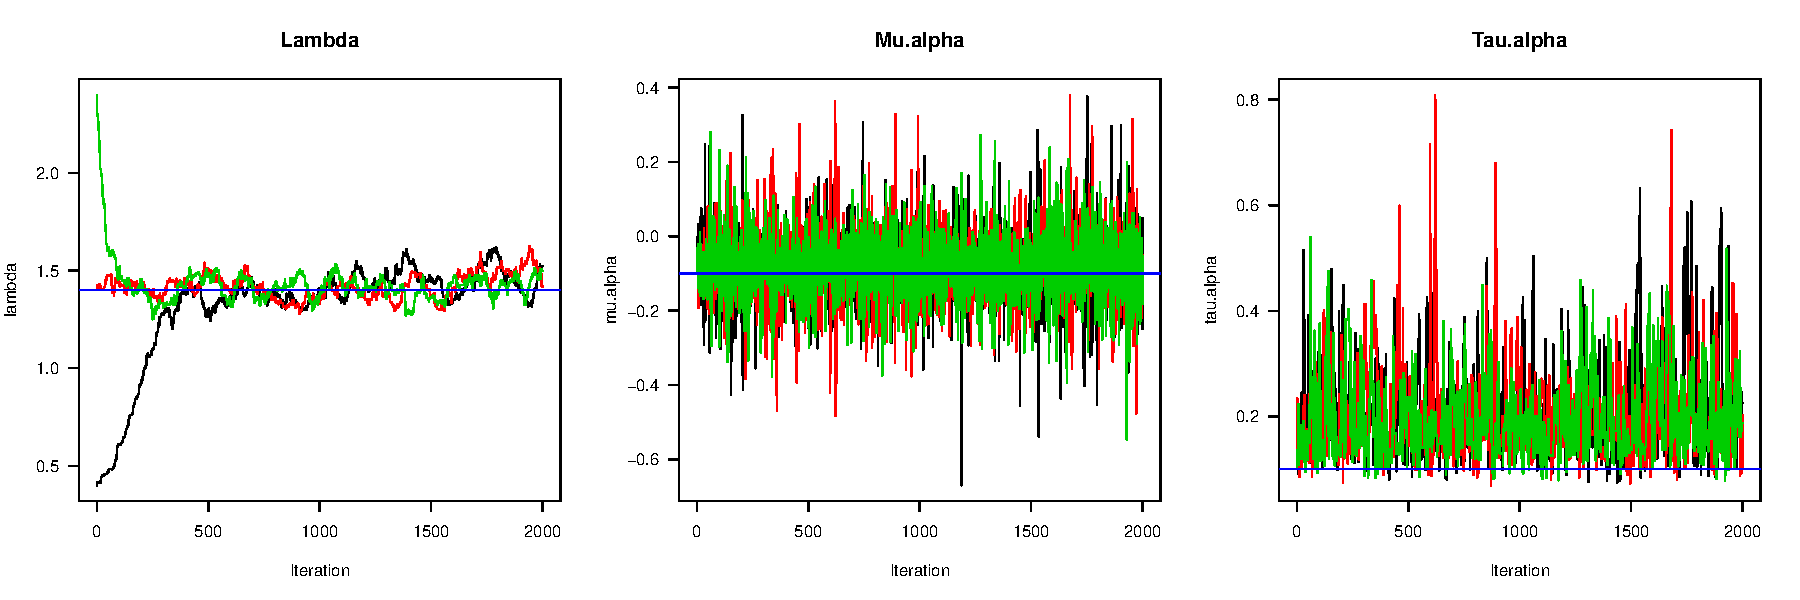
\includegraphics[width=6.0in]{fig_sim_sum1.pdf}
\caption{Simulation study results for $\lambda$, $\mu_\alpha$, and $\tau_\alpha$, where the horizontal blue lines represent the known true values of the parameters.}
\label{fig_sim_sum1}
\end{center}
\end{figure}



\section{Results}
\label{sec:results}
%Remove
Our results are based on three chains of 15,000 after a burn-in of 5,000 iterations with a jump parameter of XX and an adaption parameter of XXX. We assessed convergence by running the chain for three different starting values, 4 standard deviations above and below the historical means.The values of the Brooks, Gelman, and Rubin convergence diagnostic for each of the parameters,  were mostly below 1.1 (lambda, tau, tau.arc, mu.arc), a threshold suggested by Gainerman (1997) as satisfactory. We noticed that some of our samples stabilized after under 5,000 iterations, but a strong autocorrelation is present, such as with tau. 


\subsection{Trace Plots of Key Parameters}

\begin{figure}[htbp]
\begin{center}
\includegraphics[width=5.0in]{fig_lamba_spatialcov.pdf}
\end{center}
\end{figure}


%\includegraphics[width=6.0in]{Posterior_pwet_series8.pdf}
%\includegraphics[width=6.0in]{Posterior_pwet_series9.pdf}
%\caption{Simulation study results for $\lambda$, $\mu_\alpha$, and $\tau_\alpha$, where the horizontal blue lines represent the known true values of the parameters.}
%\label{Posterior}




\section{Discussion}
\label{sec:discuss}




\end{document}


\hspace{0.3in} $Y_{stj} = 1(Z_{stj} > 0),$\\
\vspace{0.08in}
\hspace{0.3in} $Z_{stj} \sim N(W_{st} + \alpha_s X^\text{ARC}_{sj}, \tau_s^2),$\\
\vspace{0.08in}
\hspace{0.5in} $\bW_t \sim N_S(\bX_t \bbeta, \bR),$\\
\vspace{0.08in}
\hspace{0.7in} $\beta_{ps} \sim N(\mu_p, \sigma^2_p),$\\
\vspace{0.08in}
\hspace{0.7in} $\bR=\{r_{ik}\}$, $r_{ii}=1$, $r_{ik} = \exp(-\lambda d_{ik}), \hspace{1in} \text{for $i,k \in (1,..,S)$}$\\
\vspace{0.08in}
\hspace{0.7in} $\bX_t = (1,t,\sin(2\pi t \omega_1), \cos(2\pi t \omega_1),...),$\\
\vspace{0.08in}
\hspace{0.5in} $\alpha_s \sim N(\mu_\alpha, \tau^2_\alpha),$\\
\vspace{0.08in}
where we use relatively flat priors for $\tau$, $\mu_p$, $\sigma_p$, $\lambda$, $\mu_\alpha$, and $\tau_\alpha$.


We model our observed rainfall as the part of this continuous distribution that can go below zero. 

So in the off season--if our rainfall is positive going up to 15 mm, we are pretending that we have t distribution for each site, and we are imagining that we have some t-distribution down here that is centered around -10 probably, and it never gets above zero so we never see anything. And then over the course of the year we have a t-distribution that's centered around -2, and some days we observe rainfall. And then for other months it's above zero. So we model this latent rainfall throughout. It's the random variable, btu we are modeling like it's coming from this continuous thing. 


#truncated vs censored discussion 
We should read the Sanso, based on a latent Gaussian process. They don't go into great lengths. I guess you could think of the negative rainfall as there's some underlying process still ocurring that generates the probability of there not being rainfall. But really, it's just for convenience. It's convenvient to esimate a covariance matrix when it's a continuous multivariate normal. 
We know we have covariances in our observed rainfall. In two places in ADiha you're more likely to have raifnall in one if you have rainfall in another. IT's just easier to measure correlation if it's continuous based on the level of W, not on the level of Y. 

